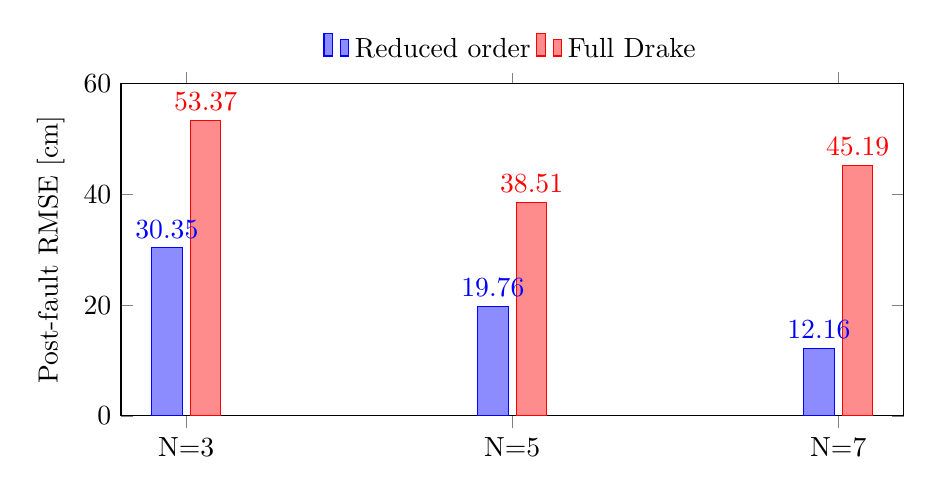
\begin{tikzpicture}
\begin{axis}[
  width=0.95\linewidth,
  height=5.8cm,
  ybar=3pt,
  bar width=11pt,
  ymin=0,
  ymax=60,
  ylabel={Post-fault RMSE [cm]},
  symbolic x coords={N=3,N=5,N=7},
  xtick=data,
  legend style={at={(0.5,1.03)}, anchor=south, legend columns=2, draw=none},
  nodes near coords,
  nodes near coords align={vertical}
]
\addplot+[fill=blue!45] coordinates {(N=3,30.35) (N=5,19.76) (N=7,12.16)};
\addplot+[fill=red!45] coordinates {(N=3,53.37) (N=5,38.51) (N=7,45.19)};
\legend{Reduced order,Full Drake}
\end{axis}
\end{tikzpicture}